\chapter{Tecnología Elegida} \label{cap4}
%\addcontentsline{toc}{chapter}{Tecnología Elegida}

\begin{flushright}
\begin{minipage}{7.85cm}
    {\em Cualquier tecnología lo suficientemente avanzada es indistinguible de
    la magia.} \\ Arthur C. Clarke
\end{minipage}
\end{flushright}

\vspace*{5mm}

\section{Licencias}

Para este proyecto vamos a usar la licencia GPL (Licencia Pública General de
GNU) en su versión 3 o posterior, escrita y mantenida por la FSF\footnote{Free
Software Foundation: \url{http://www.fsf.org/}}. El texto legal se puede
encontrar en el \hyperref[ap1]{Apéndice primero}.

Al colocar el simulador bajo esta licencia nos tenemos que asegurar que todas
las librerías que utilicemos estén bajo licencias compatibles con la nuestra. A
continuación sigue un gráfico con la relación de compatibilidad de otras
licencias libres con la GPL v3.

\begin{figure}[H]
 \centering
 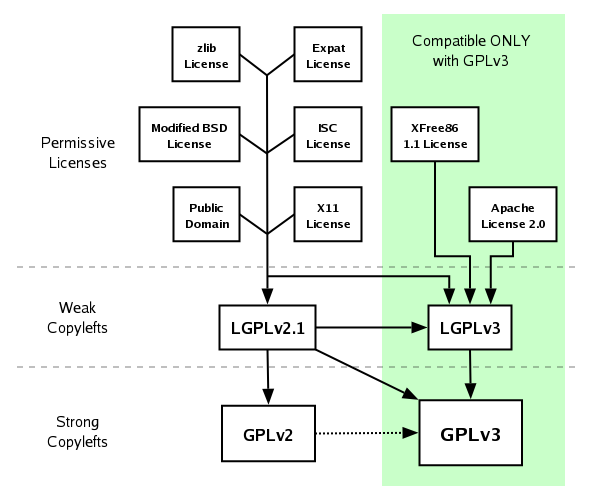
\includegraphics[width=120mm]{figuras/cap4/gplv3_comp.png}
 \caption{Compatibilidad de otras licencias libres con la GPL v3}
\end{figure}

\section{JADE}

La plataforma JADE (Java Agent DEvelopment Framework) es la escogida para el
desarrollo del simulador. El objetivo principal de esta plataforma es la
simplificación del desarrollo de sistemas multiagentes, siguiendo a su vez los
estándares de comunicación entre sistemas de la FIPA\footnote{Foundation for
Intelligent Physical Agents: \url{http://www.fipa.org/}}. FIPA es una
organización internacional sin ánimo de lucro dedicada a establecer un marco
común y genérico, para el desarrollo de agentes y sistemas multiagente.

\begin{figure}[H]
 \centering
 
\includegraphics[width=30mm]{figuras/cap4/jade.png}
 \caption{Logo de JADE}
\end{figure}

JADE está desarrollado y mantenido por Telecom
Italia\footnote{\url{http://jade.tilab.com/}}, y es una plataforma para el
desarrollo de sistemas multiagentes.

JADE puede ser considerado como un ``middleware'' que comporta una plataforma de
agentes y un entorno de desarrollo. Al utilizar JADE el desarrollador sólo tiene
que concentrarse en los agentes que escriba, el resto de aspectos del sistema
están ya resueltos, tales como el intercambio de mensajes, la búsqueda de
agentes, el ciclo de vida de estos, etc. Además está escrita en Java, lo que
aumenta la portabilidad a múltiples entornos de ejecución frente otros lenguajes
de programación.

Dado que nuestro proyecto hace uso de la licencia \hyperref[ap1]{GPL v3}, es
vital que el software que utilicemos sea también libre y esté bajo una licencia
compatible. En concreto JADE usa la licencia LGPL\footnote{Licencia Pública
General Reducida de GNU:\\
\hspace*{7mm}\url{http://www.gnu.org/licenses/old-licenses/lgpl-2.0.html}} v2.

Además de ser Software Libre, JADE tiene también la virtud de cumplir con la
especificación completa de la FIPA. Cumplir con dichos estándares es muy
importante para que sea posible la interacción entre sistemas multiagentes, y
que el proyecto no sea un entorno cerrado sin capacidad de comunicación.

Por todos estos motivos hemos escogido esta tecnología de agentes. El hecho de
utilizar JADE nos condiciona a utilizar Java como lenguaje y plataforma de
desarrollo para el proyecto. El resto de librerías y paquetes que utilizamos, y
que describimos en los siguientes apartados, están pues escritos en este
lenguaje.

\subsection{Arquitectura FIPA}

La arquitectura que sigue JADE ha sido desarrollada por FIPA con el objetivo de
permitir la construcción de sistemas multigente que se integren entre sí en un
entorno de computación particular. Adicionalmente podrían interoperar con
sistemas construidos con diferente tecnología pero que también sigan estas
especificaciones, todo ello con el mínimo esfuerzo.

\begin{figure}[H]
 \centering
 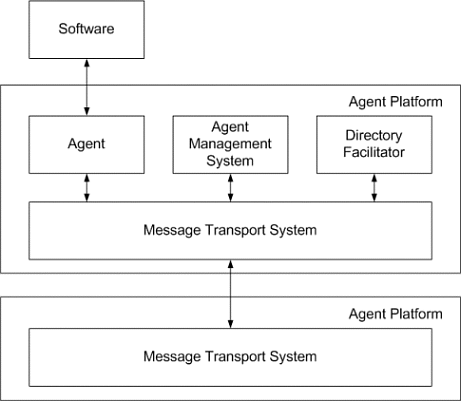
\includegraphics[width=100mm]{figuras/cap4/fipa.png}
 \caption{Arquitectura de la plataforma FIPA}
\end{figure}

FIPA establece el modelo lógico referente a la creación, destrucción, registro,
localización y comunicación de agentes. Según las especificaciones, los agentes
han de estar siempre conectados a una plataforma para poder funcionar, esto es
así debido a que su ciclo de vida es gestionado por la plataforma.

Cuando un agente se conecta a una plataforma, se produce un registro de éste
en la misma, habitualmente de manera implícita; aunque en caso de agentes
móviles que se trasladen de una plataforma a otra, por ejemplo, el registro debe
ser explícito. Este registro es necesario para que el resto de agentes puedan
localizarlo y comunicarse con él.

El estándar FIPA también define los servicios que debe proporcionar toda
plataforma de agentes, a saber:

\begin{itemize}
 \item Un sistema encargado del transporte de mensajes (Internal Platform
 Message Transport y Message Transport System).
 \item Un sistema de gestión de agentes (Agent Management System).
 \item Un servicio de directorio (Directory Facilitator).
 \item Un canal de comunicaciones para los agentes (Agent Communication
 Channel).
\end{itemize}

Cada uno de estos servicios, excepto el de transporte de mensajes, es
suministrado por agentes especializados. Esto supone que la comunicación con
ellos será mediante mensajes ACL (Agent Communication Language) y utilizando una
ontología definida para dicho servicio.

\subsubsection{Agent Management System}

El Agent Management System (AMS) es el elemento de gestión principal, tiene una
visión global sobre todo el sistema y todos sus agentes. El identificador (AID:
Agent IDentifier) es único y reservado, y viene establecido directamente por la
FIPA.

La utilidad del AMS viene determinada por los servicios que ofrece. Entre ellos
está el controlar el ciclo de vida de los agentes, por lo que ofrece mecanismos
para la creación, destrucción y control del cambio de estado de estos. El ciclo
de vida de un agente establecido por la FIPA está representado en la siguiente
figura:

\begin{figure}[H]
 \centering
 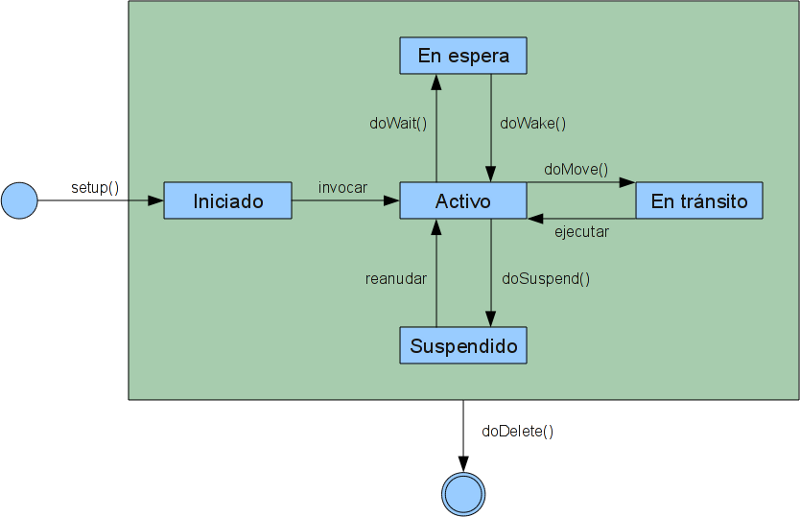
\includegraphics[width=130mm]{figuras/cap4/fipa_agent.png}
 \caption{Ciclo de vida de un agente FIPA}
\end{figure}

Además, el AMS supervisa los permisos de los agentes que registran en la
plataforma, por lo que juega un papel importante en el control de la movilidad
de los agentes.

Otras de las tareas que corresponden al AMS son la gestión de los recursos
compartidos, del canal de comunicación y del servicio de nombres (ANS: Agent
Name Service) -también conocido como ``Servicio de Páginas Blancas''-. Éste
último servicio permite a los agentes buscar por nombre a otro agente dentro de
la plataforma, y obtener la dirección de transporte real de dicho agente.

\subsubsection{Directory Facilitator}

Este agente proporciona un método para que el resto de agentes puedan registrar
sus descripciones y/o servicios, y juega un papel muy relevante dentro de la
plataforma FIPA. De esta forma se posibilita que otros agentes puedan buscar
agentes por servicios, en vez de por nombre. Gracias a este mecanismo un agente
pueden encontrar y contactar con otros agentes de cuyos servicios está
necesitado, sin conocer el nombre o identificador de estos. El Directory
Facilitator (DF) es también conocido con el nombre de ``Servicio de Páginas
Amarillas''.

Cuando un agente se registra en el DF debe proporcionar la siguiente
información: su AID y una lista de servicios que requiere u ofrece. Y cuando un
agente busca un determinado servicio en el DF, obtiene el conjunto de AIDs de
los agentes que ofrecen dicho servicio. A diferencia de lo que ocurre con el
AMS, un agente no está obligado a registrarse en el DF -el registro en el AMS
es, habitualmente, automático-.

El identificador (AID) del agente DF, al igual que el del AMS, es único y
reservado, y está establecido de antemano por la FIPA.

\subsubsection{Agent Communication Channel}

El Agent Communication Channel (ACC) es el elemento encargado de la gestión del
envío de mensajes entre los agentes de una plataforma, e incluso entre distintas
plataformas; por ello, todos los agentes han de tener acceso a un ACC.

Su misión principal es el direccionamiento de los mensajes -que están escritos
en ACL, comentado en el siguiente apartado-. El flujo es el siguiente:

\begin{enumerate}
 \item El agente emisor entrega el mensaje al ACC de su plataforma.
 \item El ACC de la plataforma emisora entrega el mensaje al ACC de la
 plataforma receptora.
 \item El segundo ACC entrega el mensaje al agente receptor.
\end{enumerate}

Todo el proceso es transparente para los agentes, que no se tienen que
preocupar de cómo llegan los mensajes que envían o reciben.

El modelo de comunicación es asíncrono, de esta manera el ACC no se bloquea
ante el envío o recepción de mensajes.

Se usan dos sistemas diferentes de transporte para los mensajes, dependiendo de
si el destino se encuentra en la misma o en otra plataforma. Para los mensajes
entre agentes de una misma plataforma, el ACC hace uso del ``Internal Platform
Message Transport'' (IPMT) que representa toda la infraestructura de
comunicaciones interna. Para la comunicación con otras plataformas, el agente
ACC dispone del ``Message Transport System'' (SMT), que hace la misma labor que
el IPMT pero a nivel externo.

\subsubsection{Agent Communication Language}

FIPA adopta como estándar el lenguaje ACL para la comunicación por mensajes.
Dicho lenguaje está basados en los ``actos del habla'', definidos en la teoría
creada por J.L. Austin\cite{Austin62}.

A diferencia del lenguaje natural, los actos del habla basan su semántica en
estados mentales, tales como creencias, deseos, intenciones, etc. Habitualmente
estos estados se pueden expresar mediante lógicas modales, lo que es muy
conveniente a la hora de trabajar en informática. Los mensajes ACL en sí mismos
definen su tipo, y por lo tanto, su semántica.

El objeto del mensaje, o expresado de otra manera, el efecto que produce en el
estado mental del emisor y del receptor, se conoce en ACL como
``Performativa''. Gracias a esta formalización es posible definir protocolos de
alto nivel, conocidos con el nombre de ``Conversaciones''.

Un mensaje ACL se compone conceptualmente de 5 partes bien diferenciadas:

\begin{description}
 \item[Performativa] O tipo de acto comunicativo. FIPA proporciona varios tipos
 como ``request'', ``query'', etc.
 \item[Emisor y receptor/es] Los identificadores (AID) de todos los agentes
 involucrados en la conversación.
 \item[Contenido] El contenido en sí del mensaje.
 \item[Descripción del contenido] De qué manera está expresado el contenido del
 mensaje, por ejemplo, siguiendo un lenguaje formal.
 \item[Control de la conversación] Parámetros que permiten a los agentes
 mantener varias conversaciones sin mezclar mensajes, por ejemplo:
 ``reply\_with'', ``in\_reply\_to'', etc.
\end{description}

\subsection{Implementación de FIPA en JADE}

Como ya hemos comentado anteriormente, JADE implementa por completo la
plataforma FIPA que acabamos de describir\cite{Corral06}. Por ejemplo, para
implementar el ACC hace uso de eventos Java para agentes en una misma máquina, y
HTTP, IIOP o Corba para comunicación entre máquinas.

En JADE la plataforma de agentes puede distribuirse entre varios contenedores,
que pueden encontrarse todos en una o en varias máquinas. En definitiva, la
plataforma puede comprender varios ordenadores, mientras que un contenedor se
ejecuta en un único ordenador, que a su vez puede ejecutar más contenedores en
paralelo (de la misma u otra plataforma).

Además de los agentes especificados por FIPA, JADE provee una interfaz gráfica
para el control y monitorización del estado de los agentes. Esta interfaz
permite, en otras acciones, crear agentes, pausarlos, matarlos, etc. El agente
que muestra esta interfaz se denomina RMA.

\begin{figure}[H]
 \centering
 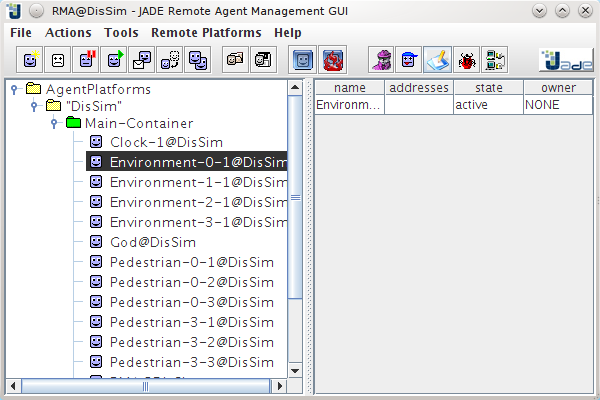
\includegraphics[width=100mm]{figuras/cap4/rma.png}
 \caption{Interfaz gráfica de usuario de JADE}
\end{figure}

Además, JADE también proporciona un agente {\em sniffer} que nos permite
``espiar'' las conversaciones entre agentes. Dicho {\em sniffer} es muy útil
para depurar la comunicación entre agentes.

\begin{figure}[H]
 \centering
 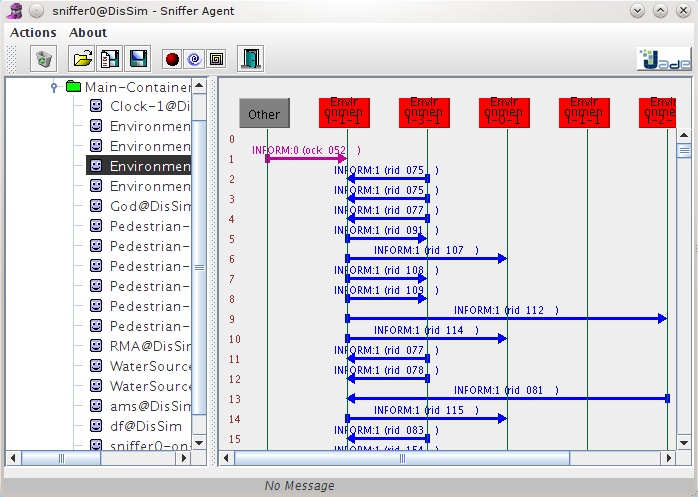
\includegraphics[width=100mm]{figuras/cap4/sniffer.png}
 \caption{Agente {\em sniffer} de JADE}
\end{figure}

\section{Java}

Java es un lenguaje de programación orientado a objetos desarrollado por Sun
Microsystems, recientemente adquirida por Oracle, a principios de los años 90.
El leitmotiv de los desarrolladores de Java era {\em write once, run anywhere},
que hace referencia a la portabilidad de un programa Java, capaz de ejecutarse
allá donde hubiera una máquina virtual, una de las características más notorias
de la plataforma.

La elección de utilizar Java viene condicionada a la elección de utilizar JADE,
que está escrito en este lenguaje.

De Java existe una implementación totalmente libre de nombre
OpenJDK\footnote{\url{http://openjdk.java.net/}}. OpenJDK soporta el 99\% de la
plataforma, y el simulador podrá ejecutarse sobre esta implementación.

\section{JAK}

JAK (Java API for KML) son un conjunto de librerías para el manejo de ficheros
KML desde Java. JAK ha sido desarrollado por Micromata
GmbH\footnote{\url{http://labs.micromata.de/display/jak/Home}}.

\begin{figure}[H]
 \centering
 
\includegraphics[width=30mm]{figuras/cap4/jak.png}
 \caption{Logo de JAK}
\end{figure}

Al igual que en el caso de {\bf JADE} es necesario que JAK sea compatible con
la licencia de nuestro proyecto, la \hyperref[ap1]{GPL v3}.
Los desarrolladores de JAK optaron por liberar las librerías bajo una licencia
BSD\footnote{Berkeley Software Distribution:\\
\hspace*{7mm}\url{http://www.opensource.org/licenses/bsd-license.php}} de 3
clausulas, o como también se la conoce, licencia BSD modificada o nueva licencia
BSD. La licencia de JAK se puede consultar en su sitio web.

Gracias a JAK podremos generar los ficheros KML con el resultado de la
simulación.

\section{Jcoord}

Para el manejo de coordenadas geográficas utilizaremos
Jcoord\footnote{\url{http://www.jstott.me.uk/jcoord/}}, un paquete de clases que
nos permitirán convertir entre formatos de coordenadas, calcular distancias,
etc. Jcoord ha sido desarrollado por Jonathan Mark Stott, y tal como se puede
consultar en su sitio web está licenciado bajo GPL v2, compatible con nuestra
\hyperref[ap1]{GPL v3}.

Además del habitual sistema de coordenadas latitud/longitud
WGS84\footnote{Sistema Geodésico Mundial 1984} soporta UTM\footnote{Sistema de
Coordenadas Universal Transversal de Mercator}.

A diferencia de {\bf JADE} o {\bf JAK}, integraremos directamente el código en
el simulador, por lo que no será una dependencia. De esta manera podremos
modificar y adaptar el paquete a nuestras necesidades.

\section{Otras librerías}

\subsection{Java CSV}

Java CSV\footnote{\url{http://sourceforge.net/projects/javacsv/}} es una
sencilla librería que facilita la escritura y lectura de ficheros de valores
separados por coma. Lo utilizaremos para escribir en ficheros los datos del
módulo de estadísticas.

La licencia de esta librería es la LGPL v2.1 o posterior, y estará integrada en
el código del proyecto por lo que no será una dependencia.

\subsection{OpenWFE}

Del proyecto OpenWFE\footnote{Open WorkFlow Engine:
\url{http://sourceforge.net/projects/openwfe/}} en realidad sólo utilizaremos
una clase. Una implementación de Wget en Java (una herramienta para descargar
ficheros de la web). La licencia de OpenWFE es una BSD de 3 clausulas.

Dicha clase estará integrada en el código del simulador por lo que OpenWFE no
será una dependencia.

\section{Servicios}

Además de las librerías comentadas hasta ahora haremos uso de algunos
servicios, como son Open Street Maps y el servicio web de elevaciones de la
USGS descritos en \hyperref[cap3]{el capítulo 3}.

\subsection{Open Street Maps}

Open Street Maps (OSM)\cite{Pinto09} permite que se le realicen peticiones GET
por HTML, y
devuelve directamente un fichero con la información solicitada en
XML\footnote{Lenguaje de Marcado Extensible: \url{http://www.w3.org/XML/}}. La
implementación de la petición será por lo tanto sencilla, aunque el tratamiento
de los datos recibidos requerirá de un procesado mucho más complejo.

\begin{figure}[H]
 \centering
 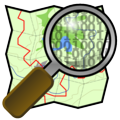
\includegraphics[width=20mm]{figuras/cap4/osm.png}
 \caption{Logo de Open Street Maps}
\end{figure}
\pagebreak
\subsection{Servicio de elevaciones de la USGS}

La U.S. Geological Survey (USGS) proporciona un método para obtener la elevación
del terreno si éste pertenece a los Estados Unidos. Este servicio consiste en un
servicio web al que se accede a través de SOAP\footnote{Simple Object Access
Protocol: \url{http://www.w3.org/TR/soap/}}. Para consumir dicho servicio hace
falta implementar un cliente, tarea que gracias a Java resulta bastante
sencilla.

Utilizaremos la herramienta {\bf wsimport} que trae Java para autogenerar el
código del cliente del servicio web, código que irá incluido en el proyecto.

\begin{figure}[H]
 \centering
 
\includegraphics[width=35mm]{figuras/cap4/usgs.png}
 \caption{Logo de la USGS}
\end{figure}

%%% Local Variables:
%%% mode: latex
%%% TeX-master: "../dissim"
%%% End: